\documentclass[12pt]{article}
\usepackage{fullpage}
\usepackage{hyperref}
\hypersetup{bookmarks=true,colorlinks=true,linkcolor=red,citecolor=blue,filecolor=magenta,urlcolor=cyan}
\usepackage{amsmath}
\usepackage{longtable}
\usepackage{booktabs}
\usepackage{caption}
\usepackage{graphics}
\title{Software Requirements Specification for solar water heating systems incorporating PCM}
\author{Thulasi Jegatheesan, Brooks MacLachlan, and Spencer Smith}
\begin{document}
\maketitle
\tableofcontents
\newpage
\section{Reference Material}
\label{Sec:RM}
This section records information for easy reference.
\subsection{Table of Units}
\label{Sec:ToU}
The unit system used throughout is SI (Syst\`{e}me International d'Unit\'{e}s). In addition to the basic units, several derived units are also used. For each unit, the table lists the symbol, a description and the SI name.
\begin{longtable*}{l l}
\toprule
Symbol & Description
\\
\midrule
m & length (metre)
\\
kg & mass (kilogram)
\\
s & time (second)
\\
${}^{\circ}C$ & temperature (centigrade)
\\
J & energy (joule)
\\
W & power (watt)
\\
\bottomrule
\label{Table:ToU}
\end{longtable*}
\subsection{Table of Symbols}
\label{Sec:ToS}
The table that follows summarizes the symbols used in this document along with their units. The choice of symbols was made to be consistent with the heat transfer literature and with existing documentation for solar water heating systems. The symbols are listed in alphabetical order.
\begin{longtable*}{l l l}
\toprule
Symbol & Description & Units
\\
\midrule
$A_{C}$ & Coil surface area & $\text{m}^{2}$
\\
$A_{in}$ & Surface area over which heat is transferred in & $\text{m}^{2}$
\\
$A_{out}$ & Surface area over which heat is transferred out & $\text{m}^{2}$
\\
$A_{P}$ & Phase change material surface area & $\text{m}^{2}$
\\
$C$ & Specific heat capacity & $\frac{\text{J}}{(\text{kg}{}^{\circ}C)}$
\\
$C^{L}$ & Specific heat capacity of a liquid & $\frac{\text{J}}{(\text{kg}{}^{\circ}C)}$
\\
$C_{P}^{L}$ & Specific heat capacity of PCM as a liquid & $\frac{\text{J}}{(\text{kg}{}^{\circ}C)}$
\\
$C^{S}$ & Specific heat capacity of a solid & $\frac{\text{J}}{(\text{kg}{}^{\circ}C)}$
\\
$C_{P}^{S}$ & Specific heat capacity of PCM as a solid & $\frac{\text{J}}{(\text{kg}{}^{\circ}C)}$
\\
$C^{V}$ & Specific heat capacity of a vapour & $\frac{\text{J}}{(\text{kg}{}^{\circ}C)}$
\\
$C_{W}$ & Specific heat capacity of water & $\frac{\text{J}}{(\text{kg}{}^{\circ}C)}$
\\
$D$ & Diameter of tank & m
\\
$E$ & Sensible heat & J
\\
$E_{Pmelt}^{init}$ & Change in heat energy in the PCM at the instant when melting begins & J
\\
$E_{P}$ & Change in heat energy in the PCM & J
\\
$E_{W}$ & Change in heat energy in the water & J
\\
$g$ & Volumetric heat generation per unit volume & $\frac{\text{W}}{\text{m}^{3}}$
\\
$h$ & Convective heat transfer coefficient & $\frac{\text{W}}{(\text{m}^{2}{}^{\circ}C)}$
\\
$h_{C}$ & Convective heat transfer coefficient between coil and water & $\frac{\text{W}}{(\text{m}^{2}{}^{\circ}C)}$
\\
$H_{f}$ & Specific latent heat of fusion & $\frac{\text{J}}{\text{kg}}$
\\
$h_{P}$ & Convective heat transfer coefficient between PCM and water & $\frac{\text{W}}{(\text{m}^{2}{}^{\circ}C)}$
\\
$L$ & Length of tank & m
\\
$m_{P}$ & Mass of phase change material & kg
\\
$m_{W}$ & Mass of water & kg
\\
$m$ & Mass & kg
\\
$\mathbf{\hat{n}}$ & Unit outward normal vector for a surface & 
\\
$q$ & Heat flux & $\frac{\text{W}}{\text{m}^{2}}$
\\
$Q$ & Latent heat & J
\\
$\mathbf{q}$ & Thermal flux vector & $\frac{\text{W}}{\text{m}^{2}}$
\\
$q_{C}$ & Heat flux into the water from the coil & $\frac{\text{W}}{\text{m}^{2}}$
\\
$q_{in}$ & Heat flux input & $\frac{\text{W}}{\text{m}^{2}}$
\\
$q_{out}$ & Heat flux output & $\frac{\text{W}}{\text{m}^{2}}$
\\
$q_{P}$ & Heat flux into the PCM from water & $\frac{\text{W}}{\text{m}^{2}}$
\\
$Q_{P}$ & Latent heat energy added to PCM & J
\\
$S$ & Surface & 
\\
$T$ & Temperature & ${}^{\circ}C$
\\
$t_{melt}^{final}$ & Time at which melting of PCM ends & s
\\
$t_{melt}^{init}$ & Time at which melting of PCM begins & s
\\
$T_{melt}^{P}$ & Melting point temperature for PCM & ${}^{\circ}C$
\\
$T_{boil}$ & Boiling point temperature & ${}^{\circ}C$
\\
$T_{C}$ & Temperature of the heating coil & ${}^{\circ}C$
\\
$T_{env}$ & Temperature of the environment & ${}^{\circ}C$
\\
$t_{final}$ & Final time & s
\\
$T_{init}$ & Initial temperature & ${}^{\circ}C$
\\
$T_{melt}$ & Melting point temperature & ${}^{\circ}C$
\\
$T_{P}$ & Temperature of the phase change material & ${}^{\circ}C$
\\
$T_{W}$ & Temperature of the water & ${}^{\circ}C$
\\
$t$ & Time & s
\\
$V$ & Volume & $\text{m}^{3}$
\\
$V_{P}$ & Volume of PCM & $\text{m}^{3}$
\\
$V_{tank}$ & Volume of the cylindrical tank & $\text{m}^{3}$
\\
$V_{W}$ & Volume of water & $\text{m}^{3}$
\\
$\Delta{}T$ & Change in temperature & ${}^{\circ}C$
\\
$\eta{}$ & ODE parameter & 
\\
$\phi{}$ & Melt fraction & 
\\
$\rho{}$ & Density & $\frac{\text{kg}}{\text{m}^{3}}$
\\
$\rho{}_{P}$ & Density of PCM & $\frac{\text{kg}}{\text{m}^{3}}$
\\
$\rho{}_{W}$ & Density of water & $\frac{\text{kg}}{\text{m}^{3}}$
\\
$\tau{}$ & Dummy variable for integration over time & s
\\
$\tau{}_{P}^{L}$ & ODE parameter for liquid PCM & s
\\
$\tau{}_{P}^{S}$ & ODE parameter for solid PCM & s
\\
$\tau{}_{W}$ & ODE parameter for water & s
\\
\bottomrule
\label{Table:ToS}
\end{longtable*}
\subsection{Abbreviations and Acronyms}
\label{Sec:AaA}
\begin{longtable*}{l l}
\toprule
Symbol & Description
\\
\midrule
A & Assumption
\\
DD & Data Definition
\\
GD & General Definition
\\
GS & Goal Statement
\\
IM & Instance Model
\\
LC & Likely Change
\\
ODE & Ordinary Differential Equation
\\
PCM & Phase Change Material
\\
PS & Physical System Description
\\
R & Requirement
\\
RHS & Right Hand Side
\\
SRS & Software Requirements Specification
\\
SWHS & Solar Water Heating System
\\
T & Theoretical Model
\\
\bottomrule
\label{Table:AaA}
\end{longtable*}
\section{Introduction}
\label{Sec:I}
Due to increasing cost, diminishing availability, and negative environmental impact of fossil fuels, there is a higher demand for renewable energy sources and energy storage technology. Solar water heating systems incorporating phase change material (PCM) use a renewable energy source and provide a novel way of storing energy. Solar water heating systems incorporating PCM improve over the traditional solar water heating systems because of their smaller size. The smaller size is possible because of the ability of PCM to store thermal energy as latent heat, which allows higher thermal energy storage capacity per unit weight.
The following section provides an overview of the Software Requirements Specification (SRS) for solar water heating systems incorporating PCM. The developed program will be referred to as Solar Water Heating System (SWHS). This section explains the purpose of this document, the scope of the system, the organization of the document and the characteristics of the intended readers.
\subsection{Purpose of Document}
\label{Sec:PoD}
The main purpose of this document is to describe the modelling of solar water heating systems incorporating PCM. The goal statements and theoretical models used in the SWHS code are provided, with an emphasis on explicitly identifying assumptions and unambiguous definitions. This document is intended to be used as a reference to provide ad hoc access to all information necessary to understand and verify the model. The SRS is abstract because the contents say what problem is being solved, but do not say how to solve it.
This document will be used as a starting point for subsequent development phases, including writing the design specification and the software verification and validation plan. The design document will show how the requirements are to be realized, including decisions on the numerical algorithms and programming environment. The verification and validation plan will show the steps that will be used to increase confidence in the software documentation and the implementation. Although the SRS fits in a series of documents that follow the so-called waterfall model, the actual development process is not constrained in any way. Even when the process is not waterfall, as Parnas and Clements [citation] point out, the most logical way to present the documentation is still to ``fake" a rational design process.
\subsection{Scope of Requirements}
\label{Sec:SoR}
The scope of the requirements is limited to thermal analysis of a single solar water heating tank incorporating PCM. Given the appropriate inputs, the code for SWHS is intended to predict the temperature and thermal energy histories for the water and the PCM. This entire document is written assuming that the substances inside the solar water heating tank are water and PCM.
\subsection{Characteristics of Intended Reader}
\label{Sec:CoIR}
Reviewers of this documentation should have a strong knowledge in heat transfer theory. A third or fourth year Mechanical Engineering course on this topic is recommended. The reviewers should also have an understanding of differential equations, as typically covered in first and second year Calculus courses. The users of SWHS can have a lower level of expertise, as explained in Section~\ref{Sec:UC}.
\subsection{Organization of Document}
\label{Sec:OoD}
The organization of this document follows the template for an SRS for scientific computing software proposed by [citation] and [citation]. The presentation follows the standard pattern for presenting goal statements, theoretical models, data definitions, and assumptions. For readers that would like a more bottom up approach, they can start reading the instance models in Section~\ref{Sec:IM} and trace back to find any additional information they require. The instance models provide the Ordinary Differential Equation (ODEs) and algebraic equations that model the solar water heating systems incorporating PCM. SWHS solves these ODEs.
The goal statements are refined to the theoretical models, and the theoretical models to the instance models. The instance models (Section~\ref{Sec:IM}) to be solved are referred to as IM1 to IM4.
\section{General System Description}
\label{Sec:GSD}
This section provides general information about the system, identifies the interfaces between the system and its environment, and describes the user characteristics and the system constraints.
\subsection{System Context}
\label{Sec:SC}
Figure~\ref{Figure::SC} shows the system context. A circle represents an external entity outside the software, the user in this case. A rectangle represents the software system itself (SWHS). Arrows are used to show the data flow between the system and its environment.
\begin{figure}
\begin{center}
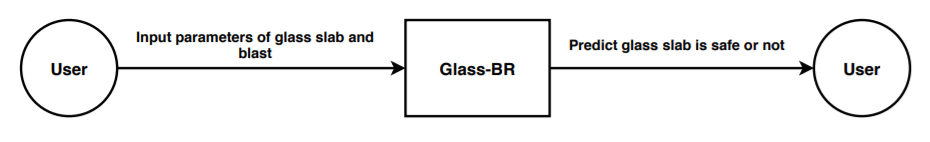
\includegraphics{SystemContextFigure.png}
\caption{Figure~\ref{Figure::SC}: System Context}
\label{Figure::SC}
\end{center}
\end{figure}
SWHS is mostly self-contained. The only external interaction is through the user interface. The responsibilities of the user and the system are as follows:
\begin{enumerate}
\item{User Responsibilities:}
\begin{enumerate}
\item{Provide the input data to the system, ensuring no errors in the data entry}
\item{Take care that consistent units are used for input variables}
\end{enumerate}
\item{SWHS Responsibilities:}
\begin{enumerate}
\item{Detect data type mismatch, such as a string of characters instead of a floating point number}
\item{Determine if the inputs satisfy the required physical and software constraints}
\item{Calculate the required outputs}
\end{enumerate}
\end{enumerate}
\subsection{User Characteristics}
\label{Sec:UC}
The end user of SWHS should have an understanding of undergraduate Level 1 Calculus and Physics.
\subsection{System Constraints}
\label{Sec:SC}
There are no system constraints.
\section{Specific System Description}
\label{Sec:SSD}
This section first presents the problem description, which gives a high-level view of the problem to be solved. This is followed by the solution characteristics specification, which presents the assumptions, theoretical models, general definitions, data definitions, and finally the instance models (ODEs) that model the solar water heating systems incorporating PCM.
\subsection{Problem Description}
\label{Sec:PD}
SWHS is a computer program developed to investigate the effect of employing PCM within a solar water heating tank.
\subsubsection{Terminology and Definitions}
\label{Sec:TaD}
This subsection provides a list of terms that are used in the subsequent sections and their meaning, with the purpose of reducing ambiguity and making it easier to correctly understand the requirements:
\begin{enumerate}
\item{Heat flux: The rate of thermal energy transfer through a given surface per unit time.}
\item{Phase Change Material (PCM): A substance that uses phase changes (such as melting) to absorb or release large amounts of heat at a constant temperature.}
\item{Specific heat capacity: The amount of energy required to raise the temperature of the unit mass of a given substance by a given amount.}
\item{Thermal conduction: The transfer of heat energy through a substance.}
\item{Transient: Changing with time.}
\end{enumerate}
\subsubsection{Physical System Description}
\label{Sec:PSD}
The physical system of SWHS, as shown in Figure~\ref{Figure:Swht,whfitwftcoahfitPfwo}, includes the following elements:
\begin{itemize}
\item[PS1:]Tank containing water.
\item[PS2:]Heating coil at bottom of tank. ($q_{C}$ represents the heat flux into the water from the coil.)
\item[PS3:]PCM suspended in tank. ($q_{P}$ represents the heat flux into the PCM from water.)
\end{itemize}
\begin{figure}
\begin{center}
\includegraphics{Tank.png}
\caption{Solar water heating tank, with heat flux into the water from the coil of $q_{C}$ and heat flux into the PCM from water of $q_{P}$}
\label{Figure:Swht,whfitwftcoahfitPfwo}
\end{center}
\end{figure}
\subsubsection{Goal Statements}
\label{Sec:GS}
Given the temperature of the heating coil, initial conditions for the temperature of the water and the temperature of the phase change material, and material properties, the goal statements are:
\begin{itemize}
\item[GS1:]Predict the temperature of the water over time.
\item[GS2:]Predict the temperature of the phase change material over time.
\item[GS3:]Predict the change in heat energy in the water over time.
\item[GS4:]Predict the change in heat energy in the PCM over time.
\end{itemize}
\subsection{Solution Characteristics Specification}
\label{Sec:SCS}
The instance models (ODEs) that govern SWHS are presented in Section~\ref{Sec:IM}. The information to understand the meaning of the instance models and their derivation is also presented, so that the instance models can be verified.
\subsubsection{Assumptions}
\label{Sec:A}
This section simplifies the original problem and helps in developing the theoretical model by filling in the missing information for the physical system. The numbers given in the square brackets refer to the theoretical model [T], general definition [GD], data definition [DD], instance model [IM], or likely change [LC], in which the respective assumption is used.
\begin{itemize}
\item[A1:]The only form of energy that is relevant for this problem is thermal energy. All other forms of energy, such as mechanical energy, are assumed to be negligible [\hyperref[T:t1ConsThermE]{Definition~T:t1ConsThermE}].
\item[A2:]All heat transfer coefficients are constant over time [GD1].
\item[A3:]The water in the tank is fully mixed, so the temperature of the water is the same throughout the entire tank [GD2, \hyperref[DD:dd2HtFluxP]{Definition~DD:dd2HtFluxP}].
\item[A4:]The temperature of the phase change material is the same throughout the volume of PCM [GD2, \hyperref[DD:dd2HtFluxP]{Definition~DD:dd2HtFluxP}, LC1].
\item[A5:]The density of water and density of PCM have no spatial variation; that is, they are each constant over their entire volume [GD2].
\item[A6:]The specific heat capacity of water, specific heat capacity of PCM as a solid, and specific heat capacity of PCM as a liquid have no spatial variation; that is, they are each constant over their entire volume [GD2].
\item[A7:]Newton's law of convective cooling applies between the heating coil and the water [\hyperref[DD:dd1HtFluxC]{Definition~DD:dd1HtFluxC}].
\item[A8:]The temperature of the heating coil is constant over time [\hyperref[DD:dd1HtFluxC]{Definition~DD:dd1HtFluxC}, LC2].
\item[A9:]The temperature of the heating coil does not vary along its length [\hyperref[DD:dd1HtFluxC]{Definition~DD:dd1HtFluxC}, LC3].
\item[A10:]Newton's law of convective cooling applies between the water and the PCM [\hyperref[DD:dd2HtFluxP]{Definition~DD:dd2HtFluxP}].
\item[A11:]The model only accounts for charging of the tank, not discharging. The temperature of the water and temperature of the phase change material can only increase, or remain constant; they do not decrease. This implies that the initial temperature (A12) is less than (or equal) to the temperature of the heating coil [IM1, LC4].
\item[A12:]The initial temperature of the water and the PCM is the same [IM1, IM2, LC5].
\item[A13:]The simulation will start with the PCM in a solid state [IM2, IM4].
\item[A14:]The operating temperature range of the system is such that the water is always in liquid state. That is, the temperature will not drop below the melting point temperature of water, or rise above its boiling point temperature [IM1, IM3].
\item[A15:]The tank is perfectly insulated so that there is no heat loss from the tank [IM1, LC6].
\item[A16:]No internal heat is generated by either the water or the PCM; therefore, the volumetric heat generation per unit volume is zero [IM1, IM2].
\item[A17:]The volume change of the PCM due to melting is negligible [IM2].
\item[A18:]The PCM is either in a liquid state or a solid state but not a gaseous state [IM2, IM4].
\item[A19:]The pressure in the tank is atmospheric, so the melting point temperature and boiling point temperature are 0${}^{\circ}C$ and 100${}^{\circ}C$, respectively [IM1, IM3].
\end{itemize}
\subsubsection{Theoretical Models}
\label{Sec:TM}
This section focuses on the general equations and laws that SWHS is based on.
~\newline
\noindent \begin{minipage}{\textwidth}
\begin{tabular}{p{0.2\textwidth} p{0.73\textwidth}}
\toprule \textbf{Refname} & \textbf{T:t1ConsThermE}
\phantomsection 
\label{T:t1ConsThermE}
\\ \midrule \\
Label & Conservation of thermal energy
\\ \midrule \\
Equation & $-\nabla{}\cdot{}\mathbf{q}+g=\rho{}C\frac{\partial{}T}{\partial{}t}$
\\ \midrule \\
Description & The above equation gives the law of conservation of energy for transient heat transfer in a material of specific heat capacity $C$ ($\frac{\text{J}}{(\text{kg}{}^{\circ}C)}$) and density, $\rho{}$ ($\frac{\text{kg}}{\text{m}^{3}}$), where $\mathbf{q}$ is the thermal flux vector ($\frac{\text{W}}{\text{m}^{2}}$), $g$ is the volumetric heat generation per unit volume ($\frac{\text{W}}{\text{m}^{3}}$), $T$ is the temperature (${}^{\circ}C$), $t$ is time (s), and $\nabla{}$ is the degree of steepness of a graph at any point. For this equation to apply, other forms of energy, such as mechanical energy, are assumed to be negligible in the system (A1).
\\ \bottomrule \end{tabular}
\end{minipage}\\
~\newline
\noindent \begin{minipage}{\textwidth}
\begin{tabular}{p{0.2\textwidth} p{0.73\textwidth}}
\toprule \textbf{Refname} & \textbf{T:t2SensHtE}
\phantomsection 
\label{T:t2SensHtE}
\\ \midrule \\
Label & Sensible heat energy
\\ \midrule \\
Equation & $E=\begin{cases}
C^{S}m*\Delta{}T, & T<T_{melt}\\
C^{L}m*\Delta{}T, & T_{melt}<T<T_{boil}\\
C^{V}m*\Delta{}T, & T_{boil}<T
\end{cases}$
\\ \midrule \\
Description & $E$ is the change in sensible heat energy (J). $C^{S}$, $C^{L}$, $C^{V}$ are the specific heat capacity of a solid, specific heat capacity of a liquid, and specific heat capacity of a vapour, respectively ($\frac{\text{J}}{(\text{kg}{}^{\circ}C)}$). $m$ is the mass (kg). $T$ is the temperature (${}^{\circ}C$), and $\Delta{}T$ is the change in temperature (${}^{\circ}C$). $T_{melt}$ and $T_{boil}$ are the melting point temperature and boiling point temperature, respectively (${}^{\circ}C$). Sensible heating occurs as long as the material does not reach a temperature where a phase change occurs. A phase change occurs if $T$=$T_{boil}$ or $T$=$T_{melt}$. If this is the case, refer to \hyperref[T:t3LatHtE]{Definition~T:t3LatHtE}, Latent heat energy.
\\ \bottomrule \end{tabular}
\end{minipage}\\
~\newline
\noindent \begin{minipage}{\textwidth}
\begin{tabular}{p{0.2\textwidth} p{0.73\textwidth}}
\toprule \textbf{Refname} & \textbf{T:t3LatHtE}
\phantomsection 
\label{T:t3LatHtE}
\\ \midrule \\
Label & Latent heat energy
\\ \midrule \\
Equation & $Q(t)=\int_{0}^{t}{\frac{dQ(\tau{})}{d\tau{}}d\tau{}}$
\\ \midrule \\
Description & $Q$ is the change in thermal energy (J), latent heat energy. FIXME: THE INTEGRAL FROM THE ABOVE EQUATION SHOULD GO HERE is the rate of change of $Q$ with respect to time $\tau{}$ (s). $t$ is the time (s) elapsed, as long as the phase change is not complete. The status of the phase change depends on the melt fraction, \hyperref[DD:dd3HtFusion]{Definition~DD:dd3HtFusion}. $T_{melt}$ and $T_{boil}$ are the melting point temperature and boiling point temperature, respectively (${}^{\circ}C$). Latent heating stops when all material has changed to the new phase.
\\ \bottomrule \end{tabular}
\end{minipage}\\
\subsubsection{General Definitions}
\label{Sec:GD}
This section collects the laws and equations that will be used in deriving the data definitions, which in turn are used to build the instance models. (General definitions are left out because they are not currently implemented in Drasil.)
Detailed derivation of simplified rate of change of temperature:
Integrating \hyperref[T:t1ConsThermE]{Definition~T:t1ConsThermE} over a volume ($V$), we have:
\begin{equation}
(-\int_{V}{\nabla{}\cdot{}\mathbf{q}dV})+\int_{V}{gdV}=\int_{V}{\rho{}C\frac{\partial{}T}{\partial{}t}dV}
\end{equation}
Applying Gauss's Divergence Theorem to the first term over the surface $S$ of the volume, with $\mathbf{q}$ as the thermal flux vector for the surface and $\mathbf{\hat{n}}$ as a unit outward normal vector for a surface:
\begin{equation}
(-\int_{S}{\mathbf{q}\cdot{}\mathbf{\hat{n}}dS})+\int_{V}{gdV}=\int_{V}{\rho{}C\frac{\partial{}T}{\partial{}t}dV}
\end{equation}
We consider an arbitrary volume. The volumetric heat generation per unit volumeis assumed constant. Then (1) can be written as:
\begin{equation}
q_{in}A_{in}-q_{out}A_{out}+gV=\int_{V}{\rho{}C\frac{\partial{}T}{\partial{}t}dV}
\end{equation}
Where $q_{in}$, $q_{out}$, $A_{in}$, and $A_{out}$ are explained in GD2. Assuming $\rho{}$, $C$ and $T$ are constant over the volume, which is true in our case by Assumptions (A3), (A4), (A5), and (A6), we have:
\begin{equation}
\rho{}CV\frac{dT}{dt}=q_{in}A_{in}-q_{out}A_{out}+gV
\end{equation}
Using the fact that $\rho{}$=$m$/$V$, (2) can be written as:
\begin{equation}
mC\frac{dT}{dt}=q_{in}A_{in}-q_{out}A_{out}+gV
\end{equation}
\subsubsection{Data Definitions}
\label{Sec:DD}
This section collects and defines all the data needed to build the instance models. The dimension of each quantity is also given.
~\newline
\noindent \begin{minipage}{\textwidth}
\begin{tabular}{p{0.2\textwidth} p{0.73\textwidth}}
\toprule \textbf{Refname} & \textbf{DD:dd1HtFluxC}
\phantomsection 
\label{DD:dd1HtFluxC}
\\ \midrule \\
Label & $q_{C}$
\\ \midrule \\
Units & $\frac{\text{W}}{\text{m}^{2}}$
\\ \midrule \\
Equation & $q_{C}$ = $h_{C}(T_{C}-T_{W}(t))$
\\ \midrule \\
Description & $q_{C}$ is the heat flux into the water from the coil\newline$h_{C}$ is the convective heat transfer coefficient between coil and water\newline$T_{C}$ is the temperature of the heating coil\newline$T_{W}$ is the temperature of the water\newline$t$ is the time
\\ \bottomrule \end{tabular}
\end{minipage}\\
~\newline
\noindent \begin{minipage}{\textwidth}
\begin{tabular}{p{0.2\textwidth} p{0.73\textwidth}}
\toprule \textbf{Refname} & \textbf{DD:dd2HtFluxP}
\phantomsection 
\label{DD:dd2HtFluxP}
\\ \midrule \\
Label & $q_{P}$
\\ \midrule \\
Units & $\frac{\text{W}}{\text{m}^{2}}$
\\ \midrule \\
Equation & $q_{P}$ = $h_{P}(T_{W}(t)-T_{P}(t))$
\\ \midrule \\
Description & $q_{P}$ is the heat flux into the PCM from water\newline$h_{P}$ is the convective heat transfer coefficient between PCM and water\newline$T_{W}$ is the temperature of the water\newline$t$ is the time\newline$T_{P}$ is the temperature of the phase change material
\\ \bottomrule \end{tabular}
\end{minipage}\\
~\newline
\noindent \begin{minipage}{\textwidth}
\begin{tabular}{p{0.2\textwidth} p{0.73\textwidth}}
\toprule \textbf{Refname} & \textbf{DD:dd3HtFusion}
\phantomsection 
\label{DD:dd3HtFusion}
\\ \midrule \\
Label & $H_{f}$
\\ \midrule \\
Units & $\frac{\text{J}}{\text{kg}}$
\\ \midrule \\
Equation & $H_{f}$ = $\frac{Q}{m}$
\\ \midrule \\
Description & $H_{f}$ is the amount of thermal energy required to completely melt a unit mass of a substance.\newline$Q$ is the latent heat energy\newline$m$ is the mass
\\ \bottomrule \end{tabular}
\end{minipage}\\
\subsubsection{Instance Models}
\label{Sec:IM}
This section transforms the problem defined in Section~\ref{Sec:PD} into one which is expressed in mathematical terms. It uses concrete symbols defined in Section~\ref{Sec:DD} to replace the abstract symbols in the models identified in Section~\ref{Sec:TM} and Section~\ref{Sec:GD}.
The goals GS1 to GS4 are solved by IM1 to IM4. The solutions for IM1 and IM2 are coupled since the solution for $T_{W}$ and $T_{P}$ depend on one another. IM3 can be solved once IM1 has been solved. The solution of IM2 and IM4 are also coupled, since the temperature of the phase change material and change in heat energy in the PCM depend on the phase change. (Instance models are left out because they are not currently implemented in Drasil.)
Derivation of the energy balance on water:
To find the rate of change of $T_{W}$, we look at the energy balance on water. The volume being considered is the volume of water $V_{W}$, which has mass of water $m_{W}$ and specific heat capacity of water, $C_{W}$. $q_{C}$ represents the heat flux into the water from the coil and $q_{P}$ represents the heat flux into the PCM from water, over coil surface area and phase change material surface area of $A_{C}$ and $A_{P}$, respectively. No heat transfer occurs to the outside of the tank, since it has been assumed to be perfectly insulated (A15). Assuming no volumetric heat generation per unit volume (A16), $g$=0. Therefore, the equation for GD2 can be written as:
\begin{equation}
m_{W}C_{W}\frac{dT_{W}}{dt}=q_{C}A_{C}-q_{P}A_{P}
\end{equation}
Using \hyperref[DD:dd1HtFluxC]{Definition~DD:dd1HtFluxC} and \hyperref[DD:dd2HtFluxP]{Definition~DD:dd2HtFluxP} for $q_{C}$ and $q_{P}$ respectively, this can be written as:
\begin{equation}
m_{W}C_{W}\frac{dT_{W}}{dt}=h_{C}A_{C}(T_{C}-T_{W})-h_{P}A_{P}(T_{W}-T_{P})
\end{equation}
Dividing (3) by $m_{W}$$C_{W}$, we obtain:
\begin{equation}
\frac{dT_{W}}{dt}=\frac{h_{C}A_{C}}{m_{W}C_{W}}(T_{C}-T_{W})-\frac{m_{P}A_{P}}{m_{W}C_{W}}(T_{W}-T_{P})
\end{equation}
Factoring the negative sign out of the second term of the RHS of Equation (4) and multiplying it by $h_{C}$$A_{C}$/$h_{C}$$A_{C}$ yields:
\begin{equation}
\frac{dT_{W}}{dt}=\frac{h_{C}A_{C}}{m_{W}C_{W}}(T_{C}-T_{W})+\frac{h_{C}A_{C}/h_{C}A_{C}h_{P}A_{P}}{m_{W}C_{W}}(T_{P}-T_{W})
\end{equation}
Which simplifies to:
\begin{equation}
\frac{dT_{W}}{dt}=\frac{h_{C}A_{C}}{m_{W}C_{W}}(T_{C}-T_{W})+\frac{h_{P}A_{P}/h_{C}A_{C}h_{C}A_{C}}{m_{W}C_{W}}(T_{P}-T_{W})
\end{equation}
Setting $\tau{}_{W}$=$m_{W}$$C_{W}$/$h_{C}$$A_{C}$ and $\eta{}$=$h_{P}$$A_{P}$/$h_{C}$$A_{C}$, Equation (5) can be written as:
\begin{equation}
\frac{dT_{W}}{dt}=\frac{1}{\tau{}_{W}}(T_{C}-T_{W})+\frac{\eta{}}{\tau{}_{W}}(T_{P}-T_{W})
\end{equation}
Finally, factoring out 1/$\tau{}_{W}$, we are left with the governing ODE for IM1:
\begin{equation}
\frac{dT_{W}}{dt}=\frac{1}{\tau{}_{W}}(T_{C}-T_{W}+\eta{}(T_{P}-T_{W}))
\end{equation}
Detailed derivation of the energy balance on the PCM during sensible heating phase:
To find the rate of change of $T_{P}$, we look at the energy balance on the PCM. The volume being considered is the volume of PCM, $V_{P}$. The derivation that follows is initially for the solid PCM. The mass of phase change material is $m_{P}$ and the specific heat capacity of PCM as a solid is $C_{P}^{S}$. The heat flux into the PCM from water is $q_{P}$ over phase change material surface area $A_{P}$. There is no heat flux output. Assuming no volumetric heat generation per unit volume (A16), $g$=0, the equation for GD2 can be written as:
\begin{equation}
m_{P}C_{P}^{S}\frac{dT_{P}}{dt}=q_{P}A_{P}
\end{equation}
Using \hyperref[DD:dd2HtFluxP]{Definition~DD:dd2HtFluxP} for $q_{P}$, this equation can be written as:
\begin{equation}
m_{P}C_{P}^{S}\frac{dT_{P}}{dt}=h_{P}A_{P}(T_{W}-T_{P})
\end{equation}
Dividing by $m_{P}$$C_{P}^{S}$ we obtain:
\begin{equation}
\frac{dT_{P}}{dt}=\frac{h_{P}A_{P}}{m_{P}C_{P}^{S}}(T_{W}-T_{P})
\end{equation}
Setting $\tau{}_{P}^{S}$=$m_{P}$$C_{P}^{S}$/$h_{P}$$A_{P}$, this can be written as:
\begin{equation}
\frac{dT_{P}}{dt}=\frac{1}{\tau{}_{P}^{S}}(T_{W}-T_{P})
\end{equation}
Equation (6) applies for the solid PCM. In the case where all of the PCM is melted, the same derivation applies, except that $C_{P}^{S}$ is replaced by $C_{P}^{L}$, and thus $\tau{}_{P}^{S}$ is replaced by $\tau{}_{P}^{L}$. Although a small change in surface area would be expected with melting, this is not included, since the volume change of the PCM with melting is assumed to be negligible (A17).
In the case where $T_{P}$=$T_{melt}^{P}$ and not all of the PCM is melted, the temperature of the phase change material does not change. Therefore, in this case d$T_{P}$/d$t$=0.
This derivation does not consider the boiling of the PCM, as the PCM is assumed to either be in a solid state or a liquid state (A18).
\subsubsection{Data Constraints}
\label{Sec:DC}
Tables 1 and 2 show the data constraints on the input and output variables, respectively. The column for physical constraints gives the physical limitations on the range of values that can be taken by the variable. The column for software constraints restricts the range of inputs to reasonable values. The constraints are conservative, to give the user of the model the flexibility to experiment with unusual situations. The column of typical values is intended to provide a feel for a common scenario. The uncertainty column provides an estimate of the confidence with which the physical quantities can be measured. This information would be part of the input if one were performing an uncertainty quantification exercise. (The tables are left out because features they should use are not yet implemented in Drasil.)
\subsubsection{Properties of a Correct Solution}
\label{Sec:PoaCS}
A correct solution must exhibit the law of conservation of energy. This means that the change in heat energy in the water should equal the difference between the total energy input from the heating coil and the energy output to the PCM. This can be shown as an equation by taking \hyperref[DD:dd1HtFluxC]{Definition~DD:dd1HtFluxC} and \hyperref[DD:dd2HtFluxP]{Definition~DD:dd2HtFluxP}, multiplying each by their respective surface area of heat transfer, and integrating each over the simulation time, as follows:
\begin{equation}
E_{W}=\int_{0}^{t}{h_{C}A_{C}(T_{C}-T_{W}(t))dt}-\int_{0}^{t}{h_{P}A_{P}(T_{W}(t)-T_{P}(t))dt}
\end{equation}
In addition, the change in heat energy in the PCM should equal the energy input to the PCM from the water. This can be expressed as
\begin{equation}
E_{P}=\int_{0}^{t}{h_{P}A_{P}(T_{W}(t)-T_{P}(t))dt}
\end{equation}
Equations (reference) and (reference) can be used as ``sanity"checks to gain confidence in any solution computed by SWHS. The relative error between the results computed by SWHS and the results calculated from the RHS of these equations should be less than 0.001% (R9).
\section{Requirements}
\label{Sec:R}
This section provides the functional requirements, the business tasks that the software is expected to complete, and the non-functional requirements, the qualities that the software is expected to exhibit.
\subsection{Functional Requirements}
\label{Sec:FR}
\begin{itemize}
\item[R1:]Input the following quantities, which define the tank parameters, material properties and initial conditions:
\end{itemize}
\begin{longtable*}{l l l}
\toprule
symbol & unit & description
\\
\midrule
$L$ & m & length of tank
\\
$D$ & m & diameter of tank
\\
$V_{P}$ & $\text{m}^{3}$ & volume of PCM
\\
$A_{P}$ & $\text{m}^{2}$ & phase change material surface area
\\
$\rho{}_{P}$ & $\frac{\text{kg}}{\text{m}^{3}}$ & density of PCM
\\
$T_{melt}^{P}$ & ${}^{\circ}C$ & melting point temperature for PCM
\\
$C_{P}^{S}$ & $\frac{\text{J}}{(\text{kg}{}^{\circ}C)}$ & specific heat capacity of PCM as a solid
\\
$C_{P}^{L}$ & $\frac{\text{J}}{(\text{kg}{}^{\circ}C)}$ & specific heat capacity of PCM as a liquid
\\
$H_{f}$ & $\frac{\text{J}}{\text{kg}}$ & specific latent heat of fusion
\\
$A_{C}$ & $\text{m}^{2}$ & coil surface area
\\
$T_{C}$ & ${}^{\circ}C$ & temperature of the heating coil
\\
$\rho{}_{W}$ & $\frac{\text{kg}}{\text{m}^{3}}$ & density of water
\\
$C_{W}$ & $\frac{\text{J}}{(\text{kg}{}^{\circ}C)}$ & specific heat capacity of water
\\
$h_{C}$ & $\frac{\text{W}}{(\text{m}^{2}{}^{\circ}C)}$ & convective heat transfer coefficient between coil and water
\\
$h_{P}$ & $\frac{\text{W}}{(\text{m}^{2}{}^{\circ}C)}$ & convective heat transfer coefficient between PCM and water
\\
$T_{init}$ & ${}^{\circ}C$ & initial temperature
\\
$t_{final}$ & s & final time
\\
\bottomrule
\label{Table:IVR}
\end{longtable*}
\begin{itemize}
\item[R2:]Use the inputs in R1 to find the mass needed for IM1 to IM4, as follows, where $V_{W}$ is the volume of water and $V_{tank}$ is the volume of the cylindrical tank.
\end{itemize}
\begin{equation}
m_{W}=V_{W}\rho{}_{W}=(V_{tank}-V_{P})\rho{}_{W}=(\frac{D}{2}L-V_{P})\rho{}_{W}
\end{equation}
\begin{equation}
m_{P}=V_{P}\rho{}_{P}
\end{equation}
\begin{itemize}
\item[R3:]Verify that the inputs satisfy the required physical constraints shown in Table 1.
\item[R4:]Output the input quantities and derived quantities in the following list: the quantities from R1, the masses from R2, $\tau{}_{W}$ (from IM1), $\eta{}$ (from IM1), $\tau{}_{P}^{S}$ (from IM2) and $\tau{}_{P}^{L}$ (from IM2).
\item[R5:]Calculate and output the temperature of the water ($T_{W}$($t$)) over the simulation time (from IM1).
\item[R6:]Calculate and output the temperature of the phase change material ($T_{P}$($t$)) over the simulation time (from IM2).
\item[R7:]Calculate and output the change in heat energy in the water ($E_{W}$($t$)) over the simulation time (from IM3).
\item[R8:]Calculate and output the change in heat energy in the PCM ($E_{P}$($t$)) over the simulation time (from IM4).
\item[R9:]Verify that the energy outputs ($E_{W}$($t$) and $E_{P}$($t$)) follow the law of conservation of energy, as outlined in Section~\ref{Sec:PoaCS}, with relative error no greater than 0.001%.
\item[R10:]Calculate and output the time at which the PCM begins to melt $t_{melt}^{init}$ (from IM2).
\item[R11:]Calculate and output the time at which the PCM stops melting $t_{melt}^{final}$ (from IM2).
\end{itemize}
\subsection{Non-functional Requirements}
\label{Sec:NR}
Given the small size, and relative simplicity, of this problem, performance is not a priority. Any reasonable implementation will be very quick and use minimal storage. Rather than performance, the priority non-functional requirements are correctness, verifiability, understandability, reusability, and maintainability.
\section{Likely Changes}
\label{Sec:LC}
\begin{itemize}
\item[LC1:]A4 - PCM is actually a poor thermal conductor, so the assumption of uniform temperature of the phase change material is not likely.
\item[LC2:]A8 - The temperature of the heating coil will change over the course of the day, depending on the energy received from the sun.
\item[LC3:]A9 - The temperature of the heating coil will actually change along its length as the water within it cools.
\item[LC4:]A11 - The model currently only accounts for charging of the tank. A more complete model would also account for discharging of the tank.
\item[LC5:]A12 - To add more flexibility to the simulation, the initial temperature of the water and the PCM could be allowed to have different values.
\item[LC6:]A15 - Any real tank cannot be perfectly insulated and will lose heat.
\end{itemize}
\section{Traceability Matrices and Graphs}
\label{Sec:TMaG}
The purpose of the traceability matrices is to provide easy references on what has to be additionally modified if a certain component is changed. Every time a component is changed, the items in the column of that component that are marked with an ``X" should be modified as well. Table~\ref{Table:TMStCBIoDS} shows the dependencies of theoretical models, general definitions, data definitions, and instance models with each other. Table~\ref{Table:TMStCBRaIM} shows the dependencies of instance models, requirements, and data constraints on each other. Table~\ref{Table:TMStCBAaOI} shows the dependencies of theoretical models, general definitions, data definitions, instance models, and likely changes on the Assumptions.
\begin{longtable}{l l l l l l l l l l l l l l}
\toprule
 & \hyperref[T:t1ConsThermE]{Definition~T:t1ConsThermE} & \hyperref[T:t2SensHtE]{Definition~T:t2SensHtE} & \hyperref[T:t3LatHtE]{Definition~T:t3LatHtE} & GD1 & GD2 & \hyperref[DD:dd1HtFluxC]{Definition~DD:dd1HtFluxC} & \hyperref[DD:dd2HtFluxP]{Definition~DD:dd2HtFluxP} & \hyperref[DD:dd3HtFusion]{Definition~DD:dd3HtFusion} & \hyperref[DD:dd3HtFusion]{Definition~DD:dd3HtFusion} & IM1 & IM2 & IM3 & IM4
\\
\midrule
\hyperref[T:t1ConsThermE]{Definition~T:t1ConsThermE} &  &  &  &  &  &  &  &  &  &  &  &  & 
\\
\hyperref[T:t2SensHtE]{Definition~T:t2SensHtE} &  &  & X &  &  &  &  &  &  &  &  &  & 
\\
\hyperref[T:t3LatHtE]{Definition~T:t3LatHtE} &  &  &  &  &  &  &  &  &  &  &  &  & 
\\
GD1 &  &  &  &  &  &  &  &  &  &  &  &  & 
\\
GD2 & X &  &  &  &  &  &  &  &  &  &  &  & 
\\
\hyperref[DD:dd1HtFluxC]{Definition~DD:dd1HtFluxC} &  &  &  & X &  &  &  &  &  &  &  &  & 
\\
\hyperref[DD:dd2HtFluxP]{Definition~DD:dd2HtFluxP} &  &  &  & X &  &  &  &  &  &  &  &  & 
\\
\hyperref[DD:dd3HtFusion]{Definition~DD:dd3HtFusion} &  &  &  &  &  &  &  &  &  &  &  &  & 
\\
\hyperref[DD:dd3HtFusion]{Definition~DD:dd3HtFusion} &  &  &  &  &  &  &  & X &  &  &  &  & 
\\
IM1 &  &  &  &  & X & X & X &  &  &  & X &  & 
\\
IM2 &  &  &  &  & X &  & X &  & X & X &  &  & X
\\
IM3 &  & X &  &  &  &  &  &  &  &  &  &  & 
\\
IM4 &  & X & X &  &  &  & X & X & X &  & X &  & 
\\
\bottomrule
\caption{Traceability Matrix Showing the Connections Between Items of Different Sections}
\label{Table:TMStCBIoDS}
\end{longtable}
\begin{longtable}{l l l l l l l l}
\toprule
 & IM1 & IM2 & IM3 & IM4 & Section~\ref{Sec:DC} & R1 & R2
\\
\midrule
IM1 &  & X &  &  &  & X & X
\\
IM2 & X &  &  & X &  & X & X
\\
IM3 &  &  &  &  &  & X & X
\\
IM4 &  & X &  &  &  & X & X
\\
R1 &  &  &  &  &  &  & 
\\
R2 &  &  &  &  &  & X & 
\\
R3 &  &  &  &  & X &  & 
\\
R4 & X & X &  &  &  & X & X
\\
R5 & X &  &  &  &  &  & 
\\
R6 &  & X &  &  &  &  & 
\\
R7 &  &  & X &  &  &  & 
\\
R8 &  &  &  & X &  &  & 
\\
R9 &  &  & X & X &  &  & 
\\
R10 &  & X &  &  &  &  & 
\\
R11 &  & X &  &  &  &  & 
\\
\bottomrule
\caption{Traceability Matrix Showing the Connections Between Requirements and Instance Models}
\label{Table:TMStCBRaIM}
\end{longtable}
\begin{longtable}{l l l l l l l l l l l l l l l l l l l l}
\toprule
 & A1 & A2 & A3 & A4 & A5 & A6 & A7 & A8 & A9 & A10 & A11 & A12 & A13 & A14 & A15 & A16 & A17 & A18 & A19
\\
\midrule
\hyperref[T:t1ConsThermE]{Definition~T:t1ConsThermE} & X &  &  &  &  &  &  &  &  &  &  &  &  &  &  &  &  &  & 
\\
\hyperref[T:t2SensHtE]{Definition~T:t2SensHtE} &  &  &  &  &  &  &  &  &  &  &  &  &  &  &  &  &  &  & 
\\
\hyperref[T:t3LatHtE]{Definition~T:t3LatHtE} &  &  &  &  &  &  &  &  &  &  &  &  &  &  &  &  &  &  & 
\\
GD1 &  & X &  &  &  &  &  &  &  &  &  &  &  &  &  &  &  &  & 
\\
GD2 &  &  & X & X & X & X &  &  &  &  &  &  &  &  &  &  &  &  & 
\\
\hyperref[DD:dd1HtFluxC]{Definition~DD:dd1HtFluxC} &  &  &  &  &  &  & X & X & X &  &  &  &  &  &  &  &  &  & 
\\
\hyperref[DD:dd2HtFluxP]{Definition~DD:dd2HtFluxP} &  &  & X & X &  &  &  &  &  & X &  &  &  &  &  &  &  &  & 
\\
\hyperref[DD:dd3HtFusion]{Definition~DD:dd3HtFusion} &  &  &  &  &  &  &  &  &  &  &  &  &  &  &  &  &  &  & 
\\
\hyperref[DD:dd3HtFusion]{Definition~DD:dd3HtFusion} &  &  &  &  &  &  &  &  &  &  &  &  &  &  &  &  &  &  & 
\\
IM1 &  &  &  &  &  &  &  &  &  &  & X & X &  & X & X & X &  &  & X
\\
IM2 &  &  &  &  &  &  &  &  &  &  &  & X & X &  &  & X & X & X & 
\\
IM3 &  &  &  &  &  &  &  &  &  &  &  &  &  & X &  &  &  &  & X
\\
IM4 &  &  &  &  &  &  &  &  &  &  &  &  & X &  &  &  &  & X & 
\\
LC1 &  &  &  & X &  &  &  &  &  &  &  &  &  &  &  &  &  &  & 
\\
LC2 &  &  &  &  &  &  &  & X &  &  &  &  &  &  &  &  &  &  & 
\\
LC3 &  &  &  &  &  &  &  &  & X &  &  &  &  &  &  &  &  &  & 
\\
LC4 &  &  &  &  &  &  &  &  &  &  & X &  &  &  &  &  &  &  & 
\\
LC5 &  &  &  &  &  &  &  &  &  &  &  & X &  &  &  &  &  &  & 
\\
LC6 &  &  &  &  &  &  &  &  &  &  &  &  &  &  & X &  &  &  & 
\\
\bottomrule
\caption{Traceability Matrix Showing the Connections Between Assumptions and Other Items}
\label{Table:TMStCBAaOI}
\end{longtable}
The purpose of the traceability graphs is also to provide easy references on what has to be additionally modified if a certain component is changed. The arrows in the graphs represent dependencies. The component at the tail of an arrow is depended on by the component at the head of that arrow. Therefore, if a component is changed, the components that it points to should also be changed. Figure~\ref{Figure:TGStCBIoDS} shows the dependencies of theoretical models, general definitions, data definitions, instance models, likely changes, and assumptions on each other. Figure~\ref{Figure:TGStCBRsIM,aDC} shows the dependencies of instance models, requirements, and data constraints on each other.
NOTE: Building a tool to automatically generate the graphical representation of the matrix by scanning the labels and reference can be future work.
\begin{figure}
\begin{center}
\includegraphics{ATrace.png}
\caption{Traceability Graph Showing the Connections Between Items of Different Sections}
\label{Figure:TGStCBIoDS}
\end{center}
\end{figure}
\begin{figure}
\begin{center}
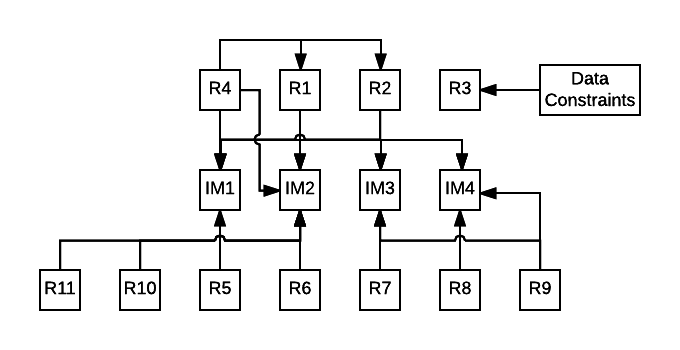
\includegraphics{RTrace.png}
\caption{Traceability Graph Showing the Connections Between Requirements, Instance Models, and Data Constraints}
\label{Figure:TGStCBRsIMsaDC}
\end{center}
\end{figure}
\end{document}
